\documentclass[conference]{IEEEtran}
\IEEEoverridecommandlockouts

% Marks
\usepackage[utf8]{inputenc}

% \DeclareUnicodeCharacter{274C}{\crossmark}
% \DeclareRobustCommand\crossmark{%
%   \unskip\nobreak\thinspace\textemdash\allowbreak\thinspace\ignorespaces}
% \DeclareUnicodeCharacter{2713}{\checkmark}

% Language (id, en)
\usepackage[english,bahasa]{babel}
\def\IEEEkeywordsname{Kata Kunci}
\def\IEEEproofname{Bukti}
\addto\extrasbahasa{
    \let\figureautorefname\undefined
    \let\tableautorefname\undefined
    \let\partautorefname\undefined
    \let\appendixautorefname\undefined
    \let\equationautorefname\undefined
    \let\Itemautorefname\undefined
    \let\chapterautorefname\undefined
    \let\sectionautorefname\undefined
    \let\subsectionautorefname\undefined
    \let\subsubsectionautorefname\undefined
    \let\paragraphautorefname\undefined
    \let\Hfootnoteautorefname\undefined
    \let\AMSautorefname\undefined
    \let\theoremautorefname\undefined
}
\newcommand{\en}[1]
    {\foreignlanguage{english}{\textit{#1}}}

% References
\usepackage[pdfborderstyle={/S/U/W 1}]{hyperref}
\usepackage{xurl}

% Listings
\usepackage{listings}
\lstset{
    frame=single,
    language=C,
    extendedchars=true,
    basicstyle=\linespread{1.2}\footnotesize\ttfamily,
}

\makeatletter
\def\lst@makecaption{%
  \def\@captype{table}%
  \@makecaption
}
\makeatother

% The preceding line is only needed to identify funding in the first footnote. If that is unneeded, please comment it out.
\usepackage{cite}
\usepackage{amsmath,amssymb,amsfonts}
\usepackage{algorithmic}
\usepackage{graphicx}
\usepackage{textcomp}
\usepackage{xcolor}
\def\BibTeX{{\rm B\kern-.05em{\sc i\kern-.025em b}\kern-.08em
    T\kern-.1667em\lower.7ex\hbox{E}\kern-.125emX}}
\begin{document}

\title{Analisis Keacakan dari Nilai \en{Hash} pada Algoritma MD dan SHA dengan Pengujian DieHard}

\author{\IEEEauthorblockN{Daniel Pintara (NIM: 13515071)}
    \IEEEauthorblockA{\textit{Teknik Informatika/Sekolah Teknik Elektro dan Informatika}\\
        \textit{Institut Teknologi Bandung}\\
        Bandung, Indonesia\\
        nieltansah@gmail.com}
}

\maketitle

\begin{abstract}
    Algoritma \en{hash} merupakan algoritma yang umum ditemukan.
    Algoritma ini berfungsi untuk melakukan verifikasi dokumen yang besar dengan mudah.
    Selain itu, algoritma ini juga dapat digunakan untuk melakukan \en{information hiding}.
    Sebagai contoh, \en{password} disimpan dalam basis data dalam bentuk nilai \en{hash}.
    Hal ini mengurangi dampak yang terjadi jika basis data tersebut diretas.
    Nilai \en{hash} yang baik harus dapat menyembunyikan pola dari nilai yang dimasukkan.
    Jika tidak, maka peretas dapat melakukan analisis terhadap nilai \en{hash} tersebut.
    Oleh karena itu, pengujian perlu dilakukan terhadap algoritma \en{hash} mengenai kemampuan algoritma tersebut dalam menyembunyikan pola.
    Pengujian ini dilakukan dengan \nameref{sec:teori:diehard} yang sudah umum digunakan untuk menilai keacakan suatu rangkaian bilangan.
\end{abstract}

\begin{IEEEkeywords}
    DieHard, nilai acak, fungsi \en{hash}, md5, sha-1, sha-256, sha3-224, sha3-512
\end{IEEEkeywords}

\section{Pendahuluan}

Algoritma \en{hash}, atau \en{message digest} merupakan algoritma yang umum digunakan.
Algoritma ini memiliki manfaat yang besar karena algoritma ini dapat menghasilkan nilai representasi dari suatu konten dokumen yang besar.
Sebagai akibatnya, algoritma ini sering digunakan sebagai penanda, apakah suatu konten dokumen merupakan konten dokumen yang sudah diubah atau belum diubah.
Selain itu, algoritma ini juga digunakan untuk menyembunyikan data rahasia, seperti PIN, \en{password}, dan lain-lain.
Penggunaan algoritma \en{hash} memungkinkan \en{password} atau PIN tersebut untuk tidak disimpan dalam bentuk plainteks, namun hanya dalam bentuk \en{hash}.
Hal ini memungkinkan pihak pengelola situs untuk memastikan bahwa \en{password} yang diberikan merupakan \en{password} yang benar walaupun pengelola situs sendiri tidak menyimpan \en{password} tersebut.
Jika terjadi peretasan terhadap basis data \en{password}, maka nilai \en{hash} dari \en{password} tersebut menjadi kurang berguna bagi \en{peretas}.
Hal ini dikarenakan peretas harus mencari nilai \en{reverse} terhadap berbagai nilai \en{hash} tersebut yang sulit untuk dilakukan.

Sebagai algoritma \en{hash} berbasis kriptografi, maka algoritma ini harus memiliki sifat \en{confusion}.
Algoritma ini juga harus dapat menyembunyikan pola umum yang terdapat pada plainteks sebelum di-\en{hash}.
Hal ini penting karena jika algoritma \en{hash} tidak mampu untuk menyembunyikan pola pada plainteks, maka peretas dapat melakukan analisis terhadap nilai \en{hash}.
Pada makalah ini, penulis akan melakukan pengujian terhadap berbagai algoritma \en{hash}.
Pengujian dilakukan dengan menggunakan \nameref{sec:teori:diehard} yang digunakan untuk mengetahui seberapa acak nilai yang dihasilkan.
Melalui teknik ini, diharapkan bahwa algoritma-algoritma \en{hash} tersebut dapat dibuktikan keacakannya.

\section{Dasar Teori}
\label{sec:teori}

\subsection{Rangkaian Pengujian DieHard}
\label{sec:teori:diehard}

\nameref{sec:teori:diehard} merupakan suatu rangkaian pengujian yang umumnya dilakukan untuk memastikan tingkat keacakan dari suatu algoritma \en{Random Number Generator (RNG)} \cite{alani2010testing}.
Pengujian ini dikembangkan oleh George Marsaglia dalam beberapa tahun yang dipublikasikan pada tahun 1995 dalam bentuk berbagai berkas dalam suatu CD-ROM. \cite{marsaglia1998diehard}
Salah satu implementasi ope
Berikut ini merupakan daftar dari subpengujian yang dilakukan pada \nameref{sec:teori:diehard} \cite{brown2013dieharder}:

\subsubsection{Jarak Ulang Tahun}
\label{sec:teori:diehard:birthday}

\begin{figure}[htbp]
    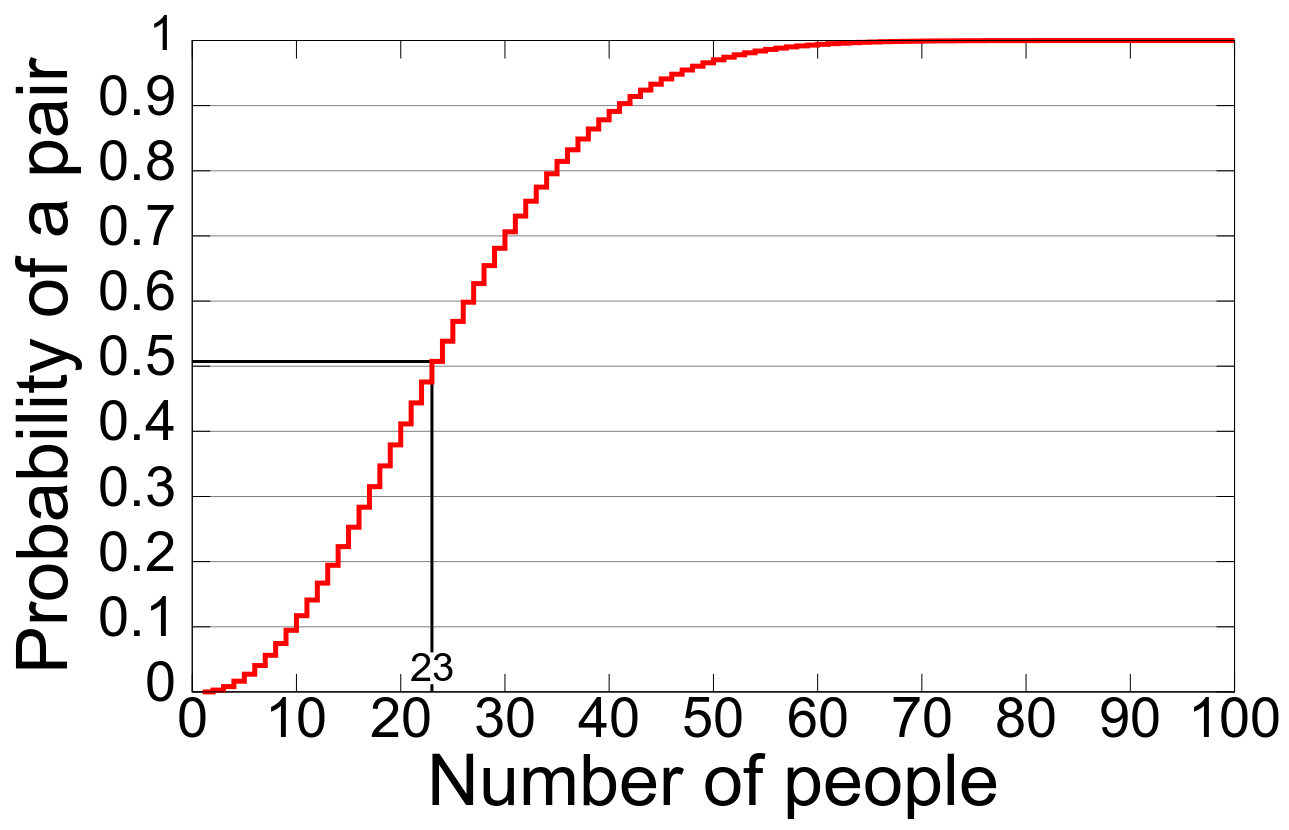
\includegraphics[width=\linewidth]{img/teori-diehard-birthday-graph.png}
    \caption{Illustrasi dari Paradoks Ulang Tahun}
    \label{fig:teori:diehard:birthday:graph}
\end{figure}

Pengujian ini dilakukan dengan cara mengambil $m$ hari ulang tahun dalam satu tahun dengan jumlah hari sebanyak $n$.
Hari ulang tahun ini diambil berdasarkan berbagai bilangan acak yang dihasilkan oleh algoritma pembangkit bilangan acak yang sedang diuji.
Pengujian ini didasari oleh paradoks ulang tahun, seperti pada \autoref{fig:teori:diehard:birthday:graph}.

Jika jarak dari berbagai hari ulang tahun terdistribusi secara exponensial asimtotik, maka pembangkit bilangan acak tersebut lolos uji.

\subsubsection{Permutasi Tumpang Tindih}

Pengujian ini disebut juga dengan pengujian OPERM5.
Pengujian ini dilakukan dengan cara mengambi satu juta bilangan acak, lalu melakukan observasi terhadap setiap lima bilangan acak yang berdekatan.

Ada $5! = 120$ cara untuk menyusun bilangan tersebut.
Jika berbagai cara tersebut muncul dengan probabilitas statistik yang sama, maka pembangkit bilangan acak tersebut lolos uji.

\subsubsection{\en{Rank} Matriks Biner}

Pengujian ini dilakukan dengan mengambil $x$-bit terkiri dari sejumlah bilangan acak yang dihasilkan oleh algoritma pembangkit bilangan acak yang sedang diuji untuk dijadikan matriks $m$x$n$.
\en{Rank} dari matriks tersebut dihitung.
Hal ini dilakukan pada banyak matriks acak yang kemudian dihitung kemunculan \en{rank} matriks dan dianalisa menggunakan pengujian Chi-square.

\subsubsection{Monyet (\en{Bitstream})}

Nama dari pengujian ini diambil dari teorema monyet tak terbatas.
Berbagai bilangan acak yang dihasilkan oleh algoritma pembangkit bilangan acak yang sedang diuji dilihat sebagai aliran bit.
Berbagai bit tersebut dikelompokkan menjadi kata, yaitu kumpulan dari berbagai bit, secara tumpang tindih.
Setelah dikelompokkan, maka perhitungan akan dilakukan terhadap kata yang hilang.

Jika jumlah dari kata yang hilang mendekati distribusi normal, maka pembangkit bilangan acak tersebut lolos uji.

\subsubsection{OPSO, OQSO dan DNA}

Pengujian OPSO dilakukan dengan memperhatikan berbagai kata dengan dua huruf dari alfabet dengan 1.024 karakter.
Setiap huruf ditentukan dengan cara mengambil 10 bit dari bilangan 32-bit yang dihasilkan oleh algoritma pembangkit bilangan acak yang sedang diuji.
Perhitungan dilakukan terhadap jumlah kata yang hilang.

Pengujian OQSO merupakan pengujian yang mirip dengan pengujian OPSO.
Pada pengujian OQSO, kata yang diperhatikan adalah berbagai kata dengan empat huruf.
Pada pengujian DNA, huruf terdiri dari C, G, A, T, yang ditentukan dari dua bit yang ditentukan dari bilangan acak yang dihasilkan oleh algoritma pembangkit bilangan acak yang sedang diuji.

\subsubsection{Jumlah Satu pada Aliran Bit}
\label{sec:teori:diehard:count1stream}

\begin{figure}[htbp]
    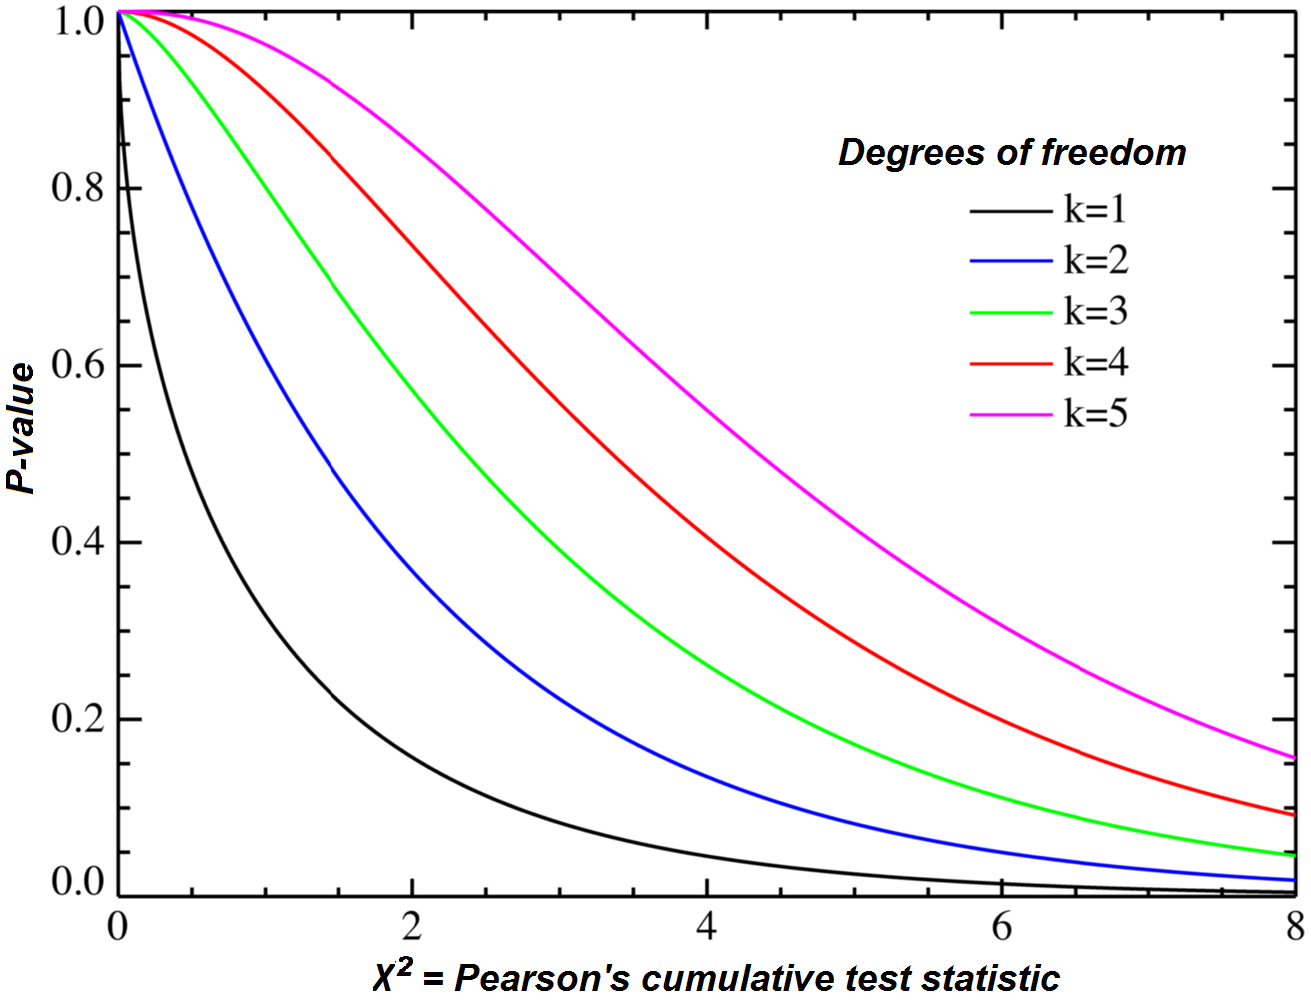
\includegraphics[width=\linewidth]{img/teori-diehard-count1stream-chi.png}
    \caption{Illustrasi dari Diagram Chi-Square}
    \label{fig:teori:diehard:count1stream:chi}
\end{figure}

Pengujian ini dilakukan dengan cara mengambil $n$ bit dari bilangan acak 32-bit.
Ada terdapat 8 kemungkinan dari jumlah 1 pada bit-bit tersebut, berdasarkan Segitiga Paskal, yaitu 1, 8, 28, 56, 70, 56, 28, 8, 1.
Perhitungan dilakukan terhadap jumlah kata, lalu dianalisa dengan menggunakan pengujian Chi-square, seperti pada \autoref{fig:teori:diehard:count1stream:chi}.

\subsubsection{Jumlah Satu pada Bit Spesifik}

Pengujian ini mirip dengan pengujian \nameref{sec:teori:diehard:count1stream}.
Pada pengujian ini, terdapat suatu monyet yang mengetik dengan probabilitas yang telah ditentukan.

Perhitungan dilakukan terhadap jumlah kata, lalu dianalisa dengan menggunakan pengujian Chi-square.

\subsubsection{Tempat Parkir}

Pengujian ini dilakukan dengan cara melakukan pemarkiran mobil secara acak berdasarkan berbagai bilangan acak yang dihasilkan oleh algoritma pembangkit bilangan acak yang sedang diuji.
Jika pemarkiran gagal karena sudah terdapat mobil, maka pemarkiran dilakukan kembali.

Perhitungan dilakukan terhadap jumlah proses pemarkiran yang terjadi serta jumlah proses pemarkiran yang gagal. Jika perhitungan tersebut mendekati distribusi dengan kurva yang mirip dengan distribusi pada bilangan acak, maka pembangkit bilangan acak tersebut lolos uji.

\subsubsection{Jarak Minimum}

Pengujian ini dilakukan dengan cara memilih titik secara acak berdasarkan berbagai bilangan acak yang dihasilkan oleh algoritma pembangkit bilangan acak yang sedang diuji.
Pemilihan titik ini memiliki batasan, yaitu hanya boleh ada pada suatu kotak yang telah ditentukan.
Jika distribusi dari jarak kuadrat tersebut mendekati rata-rata sebesar 0.995, maka pembangkit bilangan acak tersebut lolos uji.

\subsubsection{Bola 3D}

Pengujian ini dilakukan dengan cara memilih 4.000 titik acak pada suatu kubus dengan sisi sebesar 1.000.
Perhitungan dilakukan dengan cara mencari titik pusat yang memiliki jarak minimum terhadap semua titik.

Jika jarak minimum tersebut terdistribusi secara eksponensial, maka pembangkit bilangan acak tersebut lolos uji.

\subsubsection{Peremasan}

Pengujian ini dilakukan dengan cara mengalikan $2^31$ bilangan acak riil yang dihasilkan oleh algoritma pembangkit bilangan acak yang sedang diuji sampai dihasilkan bilangan satu.
Melakukan repetisi sejumlah 100.000 kali.

Jika jumlah dari bilangan acak riil tersebut memenuhi distribusi yang telah ditentukan, maka pembangkit bilangan acak tersebut lolos uji.

\subsubsection{Penjumlahan Tumpang Tindih}

Pengujian ini dilakukan dengan cara menjumlahkan bilangan acak riil yang dihasilkan oleh algoritma pembangkit bilangan acak yang sedang diuji secara tumpang tindih.

Jika hasil penjumlahan dari bilangan acak riil tersebut memenuhi distribusi dengan rata-rata dan variansi yang telah ditentukan, maka pembangkit bilangan acak tersebut lolos uji.

\subsubsection{\en{Runs}}

Pengujian ini dilakukan dengan cara membuat rangkaian panjang dari bilangan acak riil yang dihasilkan oleh algoritma pembangkit bilangan acak yang sedang diuji.
Perhitungan dilakukan terhadap bilangan menaik dan bilangan menurun.

Jika jumlah dari perilaku tersebut mengikuti distribusi tertentu, maka pembangkit bilangan acak tersebut lolos uji.

\subsubsection{\en{Craps}}

Pengujian ini dilakukan dengan memainkan permainan \en{Craps} sambil melakukan perhitungan terhadap jumlah kemenangan dan jumlah kekalahan.

Jika berbagai jumlah tersebut mengikuti distribusi tertenu, maka pembangkit bilangan acak tersebut lolos uji.

\subsection{Fungsi \en{Hash}}

\begin{figure}[htbp]
    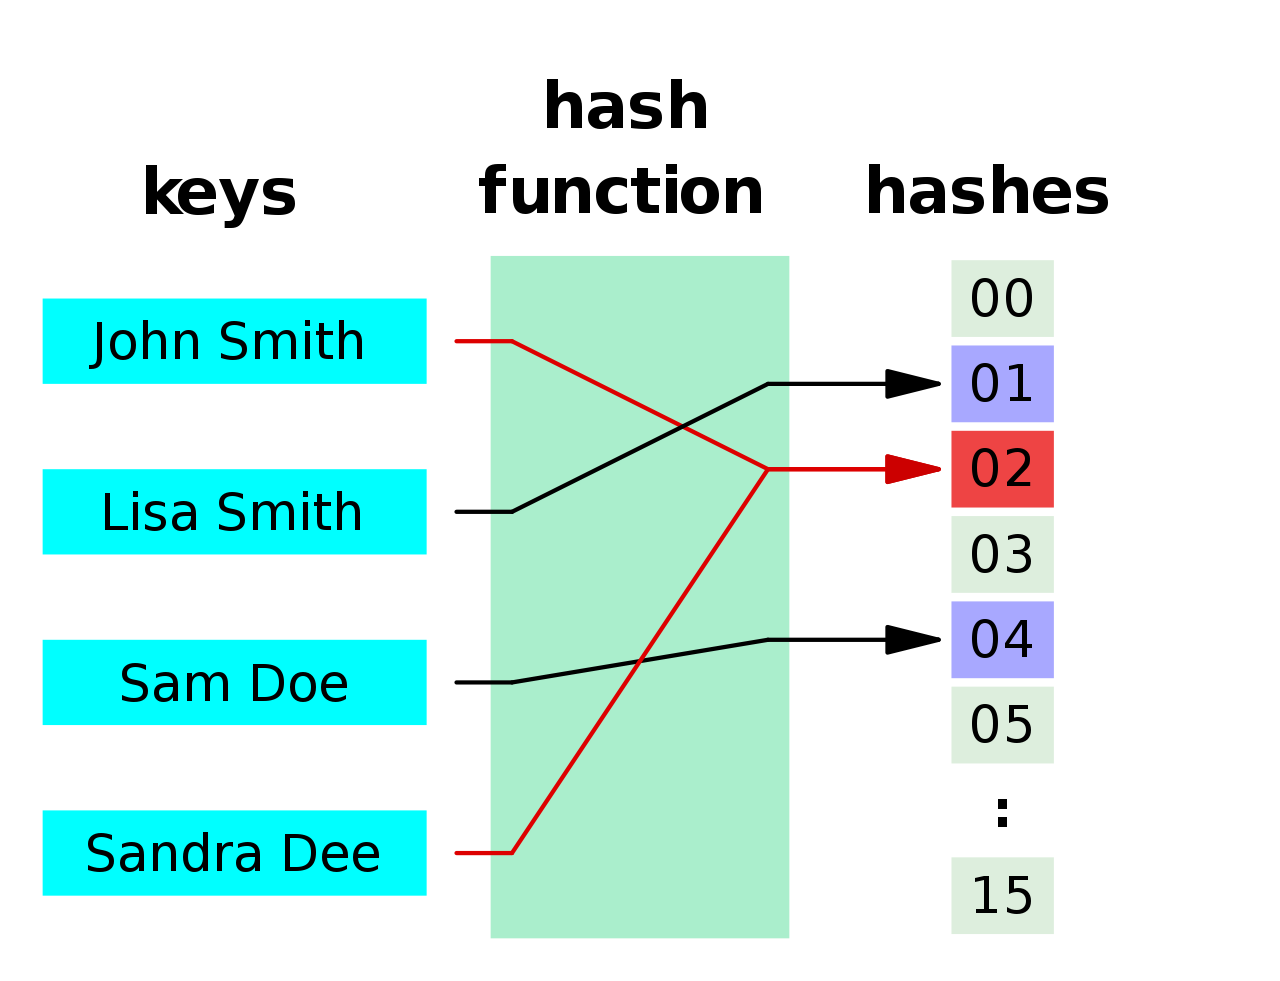
\includegraphics[width=\linewidth]{img/teori-hash-graph.png}
    \caption{Illustrasi dari Fungsi \en{Hash}}
    \label{fig:teori:hash}
\end{figure}

Fungsi \en{hash} merupakan fungsi satu arah yang berguna untuk menghasilkan representasi terhadap masukan yang diberikan. \cite{coron2005merkle}
Fungsi \en{hash} ini dapat digunakan untuk melakukan komputasi terhadap representasi suatu masukan, namun nilai tersebut tidak dapat dikembalikan kembali jika hanya diketahui nilai \en{hash} dari nilai tersebut, seperti pada \autoref{fig:teori:hash}.
Salah satu sifat yang menarik dari nilai \en{hash} adalah jika nilai yang dimasukkan berbeda sedikit, maka nilai \en{hash} yang dihasilkan berbeda jauh dari sebelumnya.

Fungsi \en{hash} banyak digunakan untuk berbagai kebutuhan, salah satu kebutuhan tersebut adalah verifikasi dokumen.
Dokumen yang ingin diverifikasi dihitung nilai \en{hash}-nya, lalu dilakukan komparasi terhadap nilai \en{hash} dari dokumen asli.
Jika dokumen tersebut memiliki nilai \en{hash} yang sama, maka dapat dipastikan bahwa kedua dokumen tersebut memiliki isi yang sama.

\subsection{Algoritma SHA-1}

\begin{figure}[htbp]
    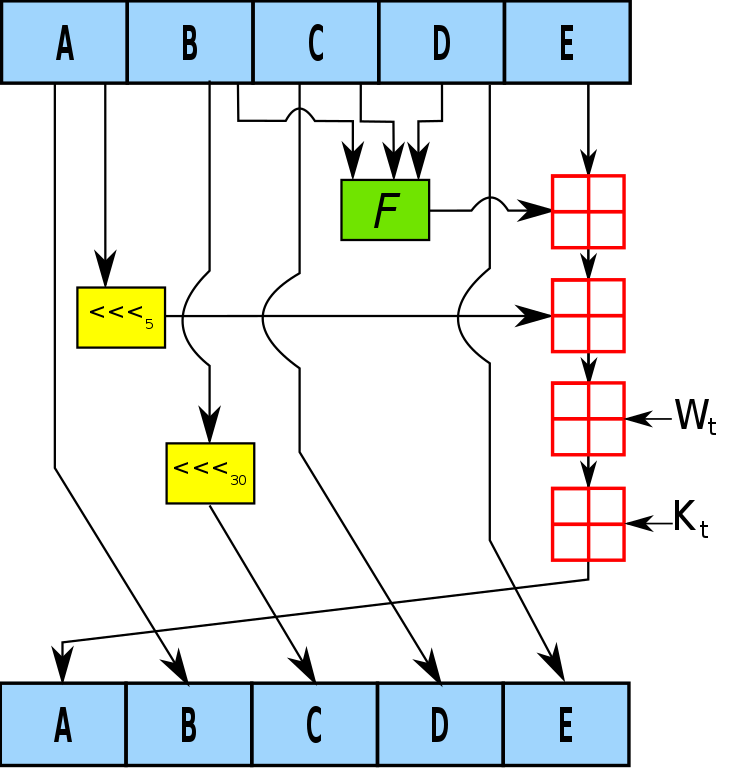
\includegraphics[width=\linewidth]{img/teori-sha1-graph.png}
    \caption{Illustrasi dari Fungsi \en{Hash} SHA-1}
    \label{fig:teori:sha1}
\end{figure}

Algoritma SHA-1 merupakan salah satu contoh dari fungsi \en{hash}.
Algoritma ini bekerja dengan cara membagi masukan menjadi blok-blok berukuran 512 bits.
Selanjutnya, algoritma ini memiliki lima nilai inisialisasi awal.
Setelah dibagi-bagi, maka untuk setiap blok, nilai tersebut akan dibagi kembali menjadi seperti pada \autoref{fig:teori:sha1}.
Masing-masing dari blok tersebut akan dilakukan perhitungan dan hasil dari perhitungan tersebut akan berkontribusi terhadap kelima nilai inisialisasi awal tersebut.
Algoritma ini menghasilkan nilai yang berbeda jika masukan yang diberikan juga berbeda.

\section{Metode Analisis}
\label{sec:analisis}

Analisis dilakukan dengan cara mengimplementasikan suatu pembangkit bilangan \en{counter}, lalu dilakukan \nameref{sec:teori:diehard} terhadap rangkaian bilangan yang dihasilkan oleh pembangkit tersebut.
Pembangkit bilangan \en{counter} merupakan pembangkit bilangan tak acak, atau deterministik, dengan \en{source code} yang tertera pada \autoref{lst:analisis:counter}.
Hal ini disebabkan karena algoritma dari pembangkit itu sendiri, yaitu hanya menambah satu dari bilangan sebelumnya.
Bilangan selanjutnya yang dihasilkan oleh pembangkit bilangan \en{counter} dapat diprediksi jika diketahui bilangan sebelumnya, lalu menambahkannya dengan satu.
\nameref{sec:teori:diehard} dilakukan untuk menguji \nameref{sec:teori:diehard} itu sendiri, bahwa \nameref{sec:teori:diehard} mampu untuk mengetahui pembangkit bilangan acak yang buruk atau yang tidak buruk.

\begin{lstlisting}[
    caption=Pembangkit Bilangan \en{Counter},
    label=lst:analisis:counter,
]
#include <stdio.h>
#include <stdint.h>

int main(void) {
    for (uint64_t i = 0;; ++i) {
        fwrite(&i, sizeof(i), 1, stdout);
    }
}
\end{lstlisting}

Setelah itu, pengujian dilanjutkan terhadap hasil dari pembangkit bilangan \en{counter} yang telah di-\en{hash} dengan berbagai macam algoritma \en{hash}, seperti pada \autoref{lst:analisis:counter-hash}.
Pengujian dilakukan dengan metode yang sama, yaitu dengan \nameref{sec:teori:diehard}.
Hal ini dilakukan untuk membuktikan apakah suatu algoritma \en{hash} tersebut dapat menutupi pola yang dihasilkan oleh pembangkit bilangan yang deterministik.

\begin{lstlisting}[
    caption=Pembangkit Bilangan \en{Counter} dengan \en{Hash},
    label=lst:analisis:counter-hash,
]
#include <stdio.h>
#include <stdint.h>
#include <openssl/evp.h>

int main(void) {
    EVP_MD_CTX *ctx;
    unsigned char* digest;
    unsigned int len;

    const EVP_MD* md = _EVP();

    if ((ctx = EVP_MD_CTX_create()) == NULL)
        return EXIT_FAILURE;
    digest =
        (uint8_t*) OPENSSL_malloc(EVP_MD_size(md));
    if (digest == NULL)
        return EXIT_FAILURE;

    int result;
    for (uint64_t i = 0;; ++i) {
        if (1 != EVP_DigestInit_ex(ctx, md, NULL))
            return EXIT_FAILURE;
        result =
            EVP_DigestUpdate(ctx, &i, sizeof(i));
        if (1 != result) return EXIT_FAILURE;
        result =
            EVP_DigestFinal_ex(ctx, digest, &len);
        if (1 != result) return EXIT_FAILURE;
        result = fwrite(digest, len, 1, stdout);
        if (1 != result) break;
    }

    return EXIT_SUCCESS;
}
\end{lstlisting}

\nameref{sec:teori:diehard} dilakukan dengan menggunakan kakas pengujian, yaitu \texttt{dieharder}.
Kakas ini sudah tersedia pada sistem operasi Linux pada umumnya, seperti pada Ubuntu, Fedora, dan lain-lain.
Kakas ini menghasilkan informasi berupa nilai \en{p-value} dari setiap pengujian yang dilakukan.
Nilai \en{p-value} baik jika nilai tersebut tidak mendekati nol ataupun satu.

\section{Pengujian dan Hasil}

Adapun hasil \nameref{sec:teori:diehard} terhadap pembangkit bilangan \en{counter} terdapat pada \autoref{tab:analisis:res-counter}.
Hasil ini menunjukkan bahwa pembangkit bilangan \en{counter} menghasilkan bilangan yang sangat deterministik.

\begin{table}[htbp]
    \caption{Hasil \nameref{sec:teori:diehard} pada Pembangkit \en{Counter}}
    \label{tab:analisis:res-counter}
    \begin{center}
        \begin{tabular}{|c|c|c|c|c|c|}
            \hline
            \textbf{name}  & \textbf{$n$} & \textbf{$t$} & \textbf{$p$} & \textbf{\en{p-value}} & \textbf{score} \\
            \hline
            birthdays      & 0            & 100          & 100          & 0.00000000            & F              \\
            operm5         & 0            & 1000000      & 100          & 0.00000000            & F              \\
            rank\_32x32    & 0            & 40000        & 100          & 0.00000000            & F              \\
            rank\_6x8      & 0            & 100000       & 100          & 0.00000000            & F              \\
            bitstream      & 0            & 2097152      & 100          & 0.00000000            & F              \\
            opso           & 0            & 2097152      & 100          & 0.00000000            & F              \\
            oqso           & 0            & 2097152      & 100          & 0.00000000            & F              \\
            dna            & 0            & 2097152      & 100          & 0.00000000            & F              \\
            count\_1s\_str & 0            & 256000       & 100          & 0.00000000            & F              \\
            count\_1s\_byt & 0            & 256000       & 100          & 0.00000000            & F              \\
            parking\_lot   & 0            & 12000        & 100          & 0.00000000            & F              \\
            2dsphere       & 2            & 8000         & 100          & 0.00000000            & F              \\
            3dsphere       & 3            & 4000         & 100          & 0.00000000            & F              \\
            squeeze        & 0            & 100000       & 100          & 0.00000000            & F              \\
            sums           & 0            & 100          & 100          & 0.00000000            & F              \\
            runs           & 0            & 100000       & 100          & 0.00000000            & F              \\
            craps          & 0            & 200000       & 100          & 0.00000000            & F              \\
            \hline
        \end{tabular}
    \end{center}
\end{table}

Adapun hasil \nameref{sec:teori:diehard} terhadap algoritma \en{hash} MD5 terdapat pada \autoref{tab:analisis:res-md5}.
Pada tabel tersebut, terlihat bahwa algoritma \en{hash} MD5 berhasil menutupi nilai deteriministik yang diberikan kepadanya dan menghasilkan hasil yang tidak deterministik.

\begin{table}[htbp]
    \caption{Hasil \nameref{sec:teori:diehard} pada Algoritma \en{Hash} MD5}
    \label{tab:analisis:res-md5}
    \begin{center}
        \begin{tabular}{|c|c|c|c|c|c|}
            \hline
            \textbf{name}  & \textbf{$n$} & \textbf{$t$} & \textbf{$p$} & \textbf{\en{p-value}} & \textbf{score} \\
            \hline
            birthdays      & 0            & 100          & 100          & 0.83493401            & P              \\
            operm5         & 0            & 1000000      & 100          & 0.13808476            & P              \\
            rank\_32x32    & 0            & 40000        & 100          & 0.49540961            & P              \\
            rank\_6x8      & 0            & 100000       & 100          & 0.96090185            & P              \\
            bitstream      & 0            & 2097152      & 100          & 0.51937065            & P              \\
            opso           & 0            & 2097152      & 100          & 0.56823387            & P              \\
            oqso           & 0            & 2097152      & 100          & 0.65456864            & P              \\
            dna            & 0            & 2097152      & 100          & 0.09236801            & P              \\
            count\_1s\_str & 0            & 256000       & 100          & 0.12818292            & P              \\
            count\_1s\_byt & 0            & 256000       & 100          & 0.79540813            & P              \\
            parking\_lot   & 0            & 12000        & 100          & 0.20530715            & P              \\
            2dsphere       & 2            & 8000         & 100          & 0.95542895            & P              \\
            3dsphere       & 3            & 4000         & 100          & 0.67579958            & P              \\
            squeeze        & 0            & 100000       & 100          & 0.48340663            & P              \\
            sums           & 0            & 100          & 100          & 0.10673786            & P              \\
            runs           & 0            & 100000       & 100          & 0.84300594            & P              \\
            runs           & 0            & 100000       & 100          & 0.66673207            & P              \\
            craps          & 0            & 200000       & 100          & 0.96596889            & P              \\
            craps          & 0            & 200000       & 100          & 0.68234665            & P              \\
            \hline
        \end{tabular}
    \end{center}
\end{table}

Adapun hasil \nameref{sec:teori:diehard} terhadap algoritma \en{hash} SHA-1 terdapat pada \autoref{tab:analisis:res-sha1}.
Pada tabel tersebut, terlihat bahwa algoritma \en{hash} SHA-1 berhasil menutupi nilai deteriministik yang diberikan kepadanya dan menghasilkan hasil yang tidak deterministik. Namun, algoritma ini memiliki kelemahan, yaitu \nameref{sec:teori:diehard} menyatakan bahwa nilai \en{p-value} dari pengujian \textbf{rank\_6x8} lemah.

\begin{table}[htbp]
    \caption{Hasil \nameref{sec:teori:diehard} pada Algoritma \en{Hash} SHA-1}
    \label{tab:analisis:res-sha1}
    \begin{center}
        \begin{tabular}{|c|c|c|c|c|c|}
            \hline
            \textbf{name}  & \textbf{$n$} & \textbf{$t$} & \textbf{$p$} & \textbf{\en{p-value}} & \textbf{score} \\
            \hline
            birthdays      & 0            & 100          & 100          & 0.90308244            & P              \\
            operm5         & 0            & 1000000      & 100          & 0.77533850            & P              \\
            rank\_32x32    & 0            & 40000        & 100          & 0.99013873            & P              \\
            rank\_6x8      & 0            & 100000       & 100          & 0.99931466            & W              \\
            bitstream      & 0            & 2097152      & 100          & 0.26177806            & P              \\
            opso           & 0            & 2097152      & 100          & 0.94065883            & P              \\
            oqso           & 0            & 2097152      & 100          & 0.13229571            & P              \\
            dna            & 0            & 2097152      & 100          & 0.10089652            & P              \\
            count\_1s\_str & 0            & 256000       & 100          & 0.28211098            & P              \\
            count\_1s\_byt & 0            & 256000       & 100          & 0.13779757            & P              \\
            parking\_lot   & 0            & 12000        & 100          & 0.92463763            & P              \\
            2dsphere       & 2            & 8000         & 100          & 0.56913822            & P              \\
            3dsphere       & 3            & 4000         & 100          & 0.21190329            & P              \\
            squeeze        & 0            & 100000       & 100          & 0.99487181            & P              \\
            sums           & 0            & 100          & 100          & 0.01418347            & P              \\
            runs           & 0            & 100000       & 100          & 0.83149758            & P              \\
            runs           & 0            & 100000       & 100          & 0.17257367            & P              \\
            craps          & 0            & 200000       & 100          & 0.22553601            & P              \\
            craps          & 0            & 200000       & 100          & 0.46018380            & P              \\
            \hline
        \end{tabular}
    \end{center}
\end{table}

Adapun hasil \nameref{sec:teori:diehard} terhadap algoritma \en{hash} SHA-256 terdapat pada \autoref{tab:analisis:res-sha256}.
Pada tabel tersebut, terlihat bahwa algoritma \en{hash} SHA-256 berhasil menutupi nilai deteriministik yang diberikan kepadanya dan menghasilkan hasil yang tidak deterministik.

\begin{table}[htbp]
    \caption{Hasil \nameref{sec:teori:diehard} pada Algoritma \en{Hash} SHA-256}
    \label{tab:analisis:res-sha256}
    \begin{center}
        \begin{tabular}{|c|c|c|c|c|c|}
            \hline
            \textbf{name}  & \textbf{$n$} & \textbf{$t$} & \textbf{$p$} & \textbf{\en{p-value}} & \textbf{score} \\
            \hline
            birthdays      & 0            & 100          & 100          & 0.11742983            & P              \\
            operm5         & 0            & 1000000      & 100          & 0.86730359            & P              \\
            rank\_32x32    & 0            & 40000        & 100          & 0.85362400            & P              \\
            rank\_6x8      & 0            & 100000       & 100          & 0.65607618            & P              \\
            bitstream      & 0            & 2097152      & 100          & 0.44602679            & P              \\
            opso           & 0            & 2097152      & 100          & 0.80592270            & P              \\
            oqso           & 0            & 2097152      & 100          & 0.50922885            & P              \\
            dna            & 0            & 2097152      & 100          & 0.38486042            & P              \\
            count\_1s\_str & 0            & 256000       & 100          & 0.55778969            & P              \\
            count\_1s\_byt & 0            & 256000       & 100          & 0.09707888            & P              \\
            parking\_lot   & 0            & 12000        & 100          & 0.69464262            & P              \\
            2dsphere       & 2            & 8000         & 100          & 0.35225641            & P              \\
            3dsphere       & 3            & 4000         & 100          & 0.07009520            & P              \\
            squeeze        & 0            & 100000       & 100          & 0.49526322            & P              \\
            sums           & 0            & 100          & 100          & 0.52833492            & P              \\
            runs           & 0            & 100000       & 100          & 0.55287078            & P              \\
            runs           & 0            & 100000       & 100          & 0.31233239            & P              \\
            craps          & 0            & 200000       & 100          & 0.81740715            & P              \\
            craps          & 0            & 200000       & 100          & 0.13152499            & P              \\
            \hline
        \end{tabular}
    \end{center}
\end{table}

Adapun hasil \nameref{sec:teori:diehard} terhadap algoritma \en{hash} SHA-512 terdapat pada \autoref{tab:analisis:res-sha512}.
Pada tabel tersebut, terlihat bahwa algoritma \en{hash} SHA-512 berhasil menutupi nilai deteriministik yang diberikan kepadanya dan menghasilkan hasil yang tidak deterministik.

\begin{table}[htbp]
    \caption{Hasil \nameref{sec:teori:diehard} pada Algoritma \en{Hash} SHA-512}
    \label{tab:analisis:res-sha512}
    \begin{center}
        \begin{tabular}{|c|c|c|c|c|c|}
            \hline
            \textbf{name}  & \textbf{$n$} & \textbf{$t$} & \textbf{$p$} & \textbf{\en{p-value}} & \textbf{score} \\
            \hline
            birthdays      & 0            & 100          & 100          & 0.83533667            & PASSED         \\
            operm5         & 0            & 1000000      & 100          & 0.09863312            & PASSED         \\
            rank\_32x32    & 0            & 40000        & 100          & 0.59920193            & PASSED         \\
            rank\_6x8      & 0            & 100000       & 100          & 0.84670622            & PASSED         \\
            bitstream      & 0            & 2097152      & 100          & 0.41207689            & PASSED         \\
            opso           & 0            & 2097152      & 100          & 0.20526907            & PASSED         \\
            oqso           & 0            & 2097152      & 100          & 0.63415543            & PASSED         \\
            dna            & 0            & 2097152      & 100          & 0.41552472            & PASSED         \\
            count\_1s\_str & 0            & 256000       & 100          & 0.28571988            & PASSED         \\
            count\_1s\_byt & 0            & 256000       & 100          & 0.39883190            & PASSED         \\
            parking\_lot   & 0            & 12000        & 100          & 0.18682201            & PASSED         \\
            2dsphere       & 2            & 8000         & 100          & 0.71181865            & PASSED         \\
            3dsphere       & 3            & 4000         & 100          & 0.54820023            & PASSED         \\
            squeeze        & 0            & 100000       & 100          & 0.22287221            & PASSED         \\
            sums           & 0            & 100          & 100          & 0.11454171            & PASSED         \\
            runs           & 0            & 100000       & 100          & 0.29782531            & PASSED         \\
            runs           & 0            & 100000       & 100          & 0.67427707            & PASSED         \\
            craps          & 0            & 200000       & 100          & 0.53878238            & PASSED         \\
            craps          & 0            & 200000       & 100          & 0.05479793            & PASSED         \\
            \hline
        \end{tabular}
    \end{center}
\end{table}

Adapun hasil \nameref{sec:teori:diehard} terhadap algoritma \en{hash} SHA-3 224-bit terdapat pada \autoref{tab:analisis:res-sha3-224}.
Pada tabel tersebut, terlihat bahwa algoritma \en{hash} SHA-3 224-bit berhasil menutupi nilai deteriministik yang diberikan kepadanya dan menghasilkan hasil yang tidak deterministik.

\begin{table}[htbp]
    \caption{Hasil \nameref{sec:teori:diehard} pada Algoritma \en{Hash} SHA-3 224-bit}
    \label{tab:analisis:res-sha3-224}
    \begin{center}
        \begin{tabular}{|c|c|c|c|c|c|}
            \hline
            \textbf{name}  & \textbf{$n$} & \textbf{$t$} & \textbf{$p$} & \textbf{\en{p-value}} & \textbf{score} \\
            \hline
            birthdays      & 0            & 100          & 100          & 0.27807841            & P              \\
            operm5         & 0            & 1000000      & 100          & 0.69003439            & P              \\
            rank\_32x32    & 0            & 40000        & 100          & 0.09806208            & P              \\
            rank\_6x8      & 0            & 100000       & 100          & 0.79949728            & P              \\
            bitstream      & 0            & 2097152      & 100          & 0.50073951            & P              \\
            opso           & 0            & 2097152      & 100          & 0.65394724            & P              \\
            oqso           & 0            & 2097152      & 100          & 0.99483965            & P              \\
            dna            & 0            & 2097152      & 100          & 0.73798246            & P              \\
            count\_1s\_str & 0            & 256000       & 100          & 0.24632876            & P              \\
            count\_1s\_byt & 0            & 256000       & 100          & 0.32165034            & P              \\
            parking\_lot   & 0            & 12000        & 100          & 0.37100770            & P              \\
            2dsphere       & 2            & 8000         & 100          & 0.85662011            & P              \\
            3dsphere       & 3            & 4000         & 100          & 0.41664466            & P              \\
            squeeze        & 0            & 100000       & 100          & 0.86884389            & P              \\
            sums           & 0            & 100          & 100          & 0.01668733            & P              \\
            runs           & 0            & 100000       & 100          & 0.75615543            & P              \\
            runs           & 0            & 100000       & 100          & 0.91420119            & P              \\
            craps          & 0            & 200000       & 100          & 0.22490163            & P              \\
            craps          & 0            & 200000       & 100          & 0.39888109            & P              \\
            \hline
        \end{tabular}
    \end{center}
\end{table}

Adapun hasil \nameref{sec:teori:diehard} terhadap algoritma \en{hash} SHA-3 512-bit terdapat pada \autoref{tab:analisis:res-sha3-512}.
Pada tabel tersebut, terlihat bahwa algoritma \en{hash} SHA-3 512-bit berhasil menutupi nilai deteriministik yang diberikan kepadanya dan menghasilkan hasil yang tidak deterministik. Namun, algoritma ini memiliki kelemahan, yaitu \nameref{sec:teori:diehard} menyatakan bahwa nilai \en{p-value} dari pengujian \textbf{bitstream} dan \textbf{sums} lemah.

\begin{table}[htbp]
    \caption{Hasil \nameref{sec:teori:diehard} pada Algoritma \en{Hash} SHA-3 512-bit}
    \label{tab:analisis:res-sha3-512}
    \begin{center}
        \begin{tabular}{|c|c|c|c|c|c|}
            \hline
            \textbf{name}  & \textbf{$n$} & \textbf{$t$} & \textbf{$p$} & \textbf{\en{p-value}} & \textbf{score} \\
            \hline
            birthdays      & 0            & 100          & 100          & 0.78652322            & P              \\
            operm5         & 0            & 1000000      & 100          & 0.39655149            & P              \\
            rank\_32x32    & 0            & 40000        & 100          & 0.26815124            & P              \\
            rank\_6x8      & 0            & 100000       & 100          & 0.37349891            & P              \\
            bitstream      & 0            & 2097152      & 100          & 0.99626020            & W              \\
            opso           & 0            & 2097152      & 100          & 0.78497667            & P              \\
            oqso           & 0            & 2097152      & 100          & 0.94383683            & P              \\
            dna            & 0            & 2097152      & 100          & 0.28817500            & P              \\
            count\_1s\_str & 0            & 256000       & 100          & 0.98306737            & P              \\
            count\_1s\_byt & 0            & 256000       & 100          & 0.65666122            & P              \\
            parking\_lot   & 0            & 12000        & 100          & 0.58615511            & P              \\
            2dsphere       & 2            & 8000         & 100          & 0.39285914            & P              \\
            3dsphere       & 3            & 4000         & 100          & 0.54598528            & P              \\
            squeeze        & 0            & 100000       & 100          & 0.23179402            & P              \\
            sums           & 0            & 100          & 100          & 0.00218225            & W              \\
            runs           & 0            & 100000       & 100          & 0.37486171            & P              \\
            runs           & 0            & 100000       & 100          & 0.36175524            & P              \\
            craps          & 0            & 200000       & 100          & 0.27652066            & P              \\
            craps          & 0            & 200000       & 100          & 0.78386810            & P              \\
            \hline
        \end{tabular}
    \end{center}
\end{table}

\section{Kesimpulan dan Saran}

Algoritma \en{hash} merupakan algoritma yang dapat menutupi sifat deterministik dari nilai yang dimasukkan pada algoritma tersebut.
Namun, terdapat beberapa algoritma yang menghasilkan nilai \en{hash} yang gagal dalam \nameref{sec:teori:diehard}.
Hal ini menunjukkan bahwa terdapat pola tertentu yang tidak acak, yang diketahui oleh pengujian ini.

\section{Kata Penutup}

Saya mengucapkan terima kasih kepada dosen saya, Bapak Dr. Ir. Rinaldi Munir, M. T. yang telah mengampu mata kuliah IF4020 Kriptografi selama satu semester ini.
Melalui jasa beliau berupa ilmu yang dicurahkan, maka makalah ini dapat diselesaikan dengan baik.

\bibliography{references}
\bibliographystyle{IEEEtran}

\section*{Pernyataan}

Dengan ini saya menyatakan bahwa makalah yang saya tulis ini adalah tulisan saya sendiri, bukan saduran, atau terjemahan dari makalah orang lain, dan bukan plagiasi.

\vspace{12pt}
\begin{flushright}
    Bandung, 10 Mei 2019

    \vspace{40pt}
    Daniel Pintara
\end{flushright}

\end{document}
